\documentclass{article}

% content/resources/templates/preamble.tex
\usepackage[margin=0.6in]{geometry}
\author{Milav Dabgar}
\usepackage{amsmath,amssymb,amsthm}
\usepackage{booktabs}
\usepackage{multirow}
\usepackage{xcolor}
\usepackage{tcolorbox}
\tcbuselibrary{breakable,skins}
\usepackage[colorlinks=true,linkcolor=blue]{hyperref}
\usepackage{titlesec}
\usepackage{enumitem}
\usepackage{tikz}
\usepackage{pgfplots}
\usepackage{circuitikz}
\usepackage[version=4]{mhchem}
\usepackage{longtable}
\usepackage{array}
\usepackage{float}
\usepackage{caption}
\usepackage{listings}

\lstset{
  basicstyle=\small\ttfamily,
  breaklines=true,
  breakatwhitespace=false,
  postbreak=\mbox{\textcolor{red}{$\hookrightarrow$}\space},
  float=false,
  numbers=left,
  numberstyle=\tiny\color{gray},
  numbersep=10pt,
  xleftmargin=2em,
  keywordstyle=\color{blue},
  commentstyle=\color{green!60!black},
  stringstyle=\color{purple},
  backgroundcolor=\color{gray!5},
  showstringspaces=false,
  tabsize=2,
  captionpos=b,
  keepspaces=true,
  columns=flexible
}

\pgfplotsset{compat=1.18}
\usetikzlibrary{shapes,arrows,positioning,calc,patterns,decorations.pathmorphing,decorations.markings,arrows.meta}

% Color scheme
\definecolor{headcolor}{RGB}{0,102,204}
\definecolor{keycolor}{RGB}{220,20,60}
\definecolor{solutioncolor}{RGB}{34,139,34}
\definecolor{mnemoniccolor}{RGB}{148,0,211}
\definecolor{codecolor}{RGB}{0,0,100}

% Spacing
\setlength{\parskip}{3pt}
\setlist[itemize]{nosep}
\setlist[enumerate]{nosep}

% Title formatting
\titleformat{\section}{\Large\bfseries\color{headcolor}}{\thesection}{1em}{}
\titleformat{\subsection}{\large\bfseries\color{headcolor}}{\thesubsection}{1em}{}

% Pandoc tightlist compatibility
\providecommand{\tightlist}{%
  \setlength{\itemsep}{0pt}\setlength{\parskip}{0pt}}

% Pandoc longtable compatibility
\newcounter{none}
\def\thenone{}


% content/resources/templates/english-boxes.tex

% Custom environments
\newtcolorbox{solutionbox}{
 breakable,
 enhanced,
 colback=solutioncolor!5!white,
 colframe=solutioncolor!75!black,
 fonttitle=\bfseries,
 title=Solution
}

\newtcolorbox{solutionboxnobreak}{
 colback=solutioncolor!5!white,
 colframe=solutioncolor!75!black,
 fonttitle=\bfseries,
 title=Solution
}

\newtcolorbox{keyformula}{
 breakable,
 enhanced,
 colback=keycolor!5!white,
 colframe=keycolor!75!black,
 fonttitle=\bfseries,
 title=Key Formula
}

\newtcolorbox{mnemonicboxenv}{
 breakable,
 enhanced,
 colback=mnemoniccolor!5!white,
 colframe=mnemoniccolor!75!black,
 fonttitle=\bfseries,
 title=Mnemonic
}

\newcommand{\mnemonicbox}[1]{%
  \begin{mnemonicboxenv}
    #1
  \end{mnemonicboxenv}
}


% Custom commands for GTU solutions
% This file defines semantic commands for consistent formatting

% Question command with automatic formatting
\newcommand{\question}[2]{%
  \section*{Question #1}%
  \textbf{#2}%
}

% OR question variant
\newcommand{\questionor}[2]{%
  \section*{Question #1 OR}%
  \textbf{#2}%
}

% Proper table environment with caption
\newenvironment{answertable}[1]{%
  \begin{table}[htbp]
  \centering
  \caption{#1}
}{%
  \end{table}
}

% Proper figure environment for diagrams
\newenvironment{answerdiagram}[1]{%
  \begin{figure}[htbp]
  \centering
  \caption{#1}
}{%
  \end{figure}
}

% Semantic markup for key terms
\newcommand{\keyword}[1]{\textbf{#1}}
\newcommand{\code}[1]{\texttt{#1}}
\newcommand{\classname}[1]{\texttt{#1}}
\newcommand{\methodname}[1]{\texttt{#1}}

% Proper quotation marks
\newcommand{\mnemonic}[1]{``#1''}


\title{Microwave and Radar Communication (4351103) - Summer 2025 Solution}
\date{May 16, 2025}

\begin{document}
\maketitle

\questionmarks{1(a)}{3}{List four microwave frequency bands with their frequency range and applications.}

\begin{solutionbox}
\textbf{Microwave Bands:}

\begin{answertable}{Frequency Bands}
\begin{tabulary}{\linewidth}{|L|L|L|}
\hline
\textbf{Band} & \textbf{Frequency Range} & \textbf{Applications} \\ \hline
\keyword{L-band} & 1-2 GHz & GPS, Mobile communication \\ \hline
\keyword{S-band} & 2-4 GHz & WiFi, Bluetooth, Radar \\ \hline
\keyword{C-band} & 4-8 GHz & Satellite communication \\ \hline
\keyword{X-band} & 8-12 GHz & Military radar, Weather radar \\ \hline
\end{tabulary}
\end{answertable}
\end{solutionbox}

\begin{mnemonicbox}
\mnemonic{Little Satellites Communicate eXcellently}
\end{mnemonicbox}

\questionmarks{1(b)}{4}{Explain the impedance matching process using a single stub.}

\begin{solutionbox}
\textbf{Single Stub Matching:}
Removes reflections by adding a \keyword{short-circuited stub} at specific distance from load.

\begin{answerdiagram}{Single Stub Matching}
\begin{tikzpicture}[auto, node distance=2cm]
    \node [gtu block] (source) {Source};
    \node [gtu block, right=of source] (stub_point) {Stub Position};
    \node [gtu block, right=of stub_point] (load) {Load ($Z_L$)};
    \node [gtu block, below=of stub_point] (stub) {Short Stub};

    \draw [gtu arrow] (source) -- node[above] {Line} (stub_point);
    \draw [gtu arrow] (stub_point) -- node[above] {$d$} (load);
    \draw [gtu arrow] (stub) -- node[right] {$l$} (stub_point);
\end{tikzpicture}
\end{answerdiagram}

\textbf{Process:}
\begin{enumerate}
    \item \keyword{Stub length}: Provides reactive impedance to cancel line reactance.
    \item \keyword{Stub position}: Point on line where real part of admittance is $Y_0$.
    \item \keyword{Matching condition}: Total Admittance $Y = Y_0 + jB_{line} - jB_{stub} = Y_0$.
\end{enumerate}
\end{solutionbox}

\begin{mnemonicbox}
\mnemonic{Stub Positioned for Perfect Matching}
\end{mnemonicbox}

\questionmarks{1(c)}{7}{State characteristics of lossless transmission line and obtain the general equation for a two-wire transmission line.}

\begin{solutionbox}
\textbf{Characteristics of Lossless Line:}
\begin{itemize}
    \item \keyword{No power loss}: $R = 0, G = 0$.
    \item \keyword{Constant amplitude}: No attenuation ($\alpha = 0$).
    \item \keyword{Phase delay only}: Signal is delayed but not weakened.
    \item \keyword{Standing wave pattern}: Formed due to reflections from mismatched load.
\end{itemize}

\textbf{General Equations:}
For a line with propagation constant $\gamma = \alpha + j\beta$ and characteristic impedance $Z_0$:

\keyword{Voltage Equation}:
\[ V(z) = V^+ e^{-\gamma z} + V^- e^{\gamma z} \]

\keyword{Current Equation}:
\[ I(z) = \frac{V^+}{Z_0} e^{-\gamma z} - \frac{V^-}{Z_0} e^{\gamma z} \]

Where:
\begin{itemize}
    \item $Z_0 = \sqrt{L/C}$ (for lossless line).
    \item $\gamma = j\beta$ (since $\alpha=0$).
\end{itemize}
\end{solutionbox}

\begin{mnemonicbox}
\mnemonic{Lossless Lines Love Low Loss}
\end{mnemonicbox}

\orquestionmarks{1(c)}{7}{Define standing wave. Draw and explain the standing wave pattern for short circuit and open circuit line.}

\begin{solutionbox}
\textbf{Standing Wave:}
Fixed pattern formed by the interference of \keyword{forward} and \keyword{reflected waves} traveling in opposite directions.

\begin{answerdiagram}{Standing Wave Patterns}
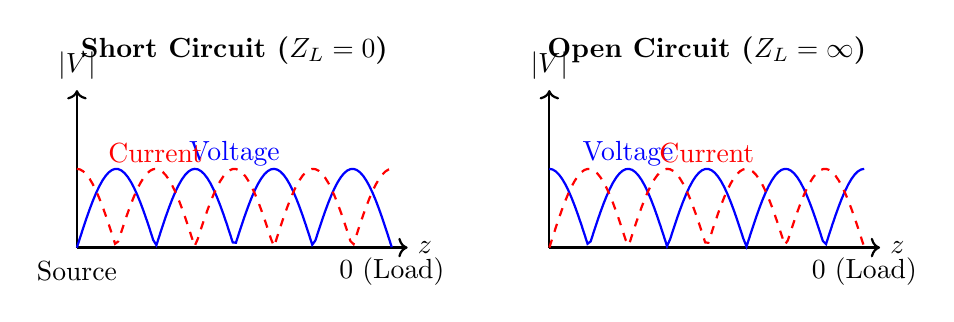
\begin{tikzpicture}
    % Short Circuit
    \begin{scope}
        \node at (2, 2.5) {\textbf{Short Circuit ($Z_L=0$)}};
        % Voltage (Min at load)
        \draw[thick, ->] (0,0) -- (4.2,0) node[right] {$z$};
        \draw[thick, ->] (0,0) -- (0,2) node[above] {$|V|$};
        \draw[blue, thick] plot[domain=0:4, samples=100] (\x, {abs(sin(180*\x))});
        \node[blue] at (2,1.2) {Voltage};
        \node at (4, -0.3) {0 (Load)};
        \node at (0, -0.3) {Source};
        
        % Current (Max at load)
        \draw[red, dashed, thick] plot[domain=0:4, samples=100] (\x, {abs(cos(180*\x))});
        \node[red] at (1,1.2) {Current};
    \end{scope}

    % Open Circuit
    \begin{scope}[xshift=6cm]
        \node at (2, 2.5) {\textbf{Open Circuit ($Z_L=\infty$)}};
        % Voltage (Max at load)
        \draw[thick, ->] (0,0) -- (4.2,0) node[right] {$z$};
        \draw[thick, ->] (0,0) -- (0,2) node[above] {$|V|$};
        \draw[blue, thick] plot[domain=0:4, samples=100] (\x, {abs(cos(180*\x))});
        \node[blue] at (1,1.2) {Voltage};
        \node at (4, -0.3) {0 (Load)};

        % Current (Min at load)
        \draw[red, dashed, thick] plot[domain=0:4, samples=100] (\x, {abs(sin(180*\x))});
        \node[red] at (2,1.2) {Current};
    \end{scope}
\end{tikzpicture}
\end{answerdiagram}

\textbf{Analysis:}
\begin{answertable}{Standing Wave Features}
\begin{tabulary}{\linewidth}{|L|L|L|}
\hline
\textbf{Condition} & \textbf{Voltage at Load} & \textbf{Current at Load} \\ \hline
\keyword{Short Circuit} & Minimum (0) & Maximum \\ \hline
\keyword{Open Circuit} & Maximum ($2V^+$) & Minimum (0) \\ \hline
\end{tabulary}
\end{answertable}
Distance between successive maxima or minima is $\lambda/2$.
\end{solutionbox}

\begin{mnemonicbox}
\mnemonic{Short Circuits Current, Open Circuits Voltage}
\end{mnemonicbox}

\questionmarks{2(a)}{3}{Draw and explain the working of Magic TEE.}

\begin{solutionbox}
\textbf{Magic TEE:}
A 4-port hybrid waveguide junction combining E-plane and H-plane Tees.

\begin{answerdiagram}{Magic TEE Structure}
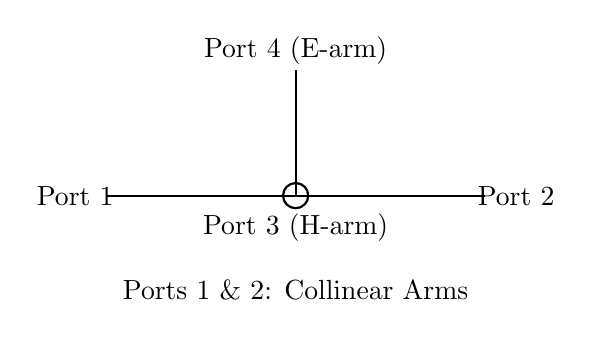
\begin{tikzpicture}[scale=0.8]
    \draw[thick] (-3,0) -- (3,0); % Main arm
    \draw[thick] (0,0) -- (0,2);  % E-arm
    \draw[thick] (0,0) circle (0.2); % H-arm representation
    
    \node at (-3.5,0) {Port 1};
    \node at (3.5,0) {Port 2};
    \node at (0,2.3) {Port 4 (E-arm)};
    \node at (0,-0.5) {Port 3 (H-arm)};
    
    \node at (0,-1.5) {Ports 1 \& 2: Collinear Arms};
\end{tikzpicture}
\end{answerdiagram}

\textbf{Working:}
\begin{itemize}
    \item \keyword{Port 3 (H-arm)}: Sum port ($P_3 \propto P_1 + P_2$). Inputs at 1 \& 2 appear in phase.
    \item \keyword{Port 4 (E-arm)}: Difference port ($P_4 \propto P_1 - P_2$). Inputs at 1 \& 2 appear $180^\circ$ out of phase.
    \item \keyword{Isolation}: No coupling between E-arm (4) and H-arm (3).
\end{itemize}
\end{solutionbox}

\begin{mnemonicbox}
\mnemonic{Magic Tee Mixes Modes}
\end{mnemonicbox}

\questionmarks{2(b)}{4}{Explain the working of Hybrid ring.}

\begin{solutionbox}
\textbf{Hybrid Ring (Rat-Race Coupler):}
A circular waveguide with 4 ports used for power splitting and summing.

\begin{answerdiagram}{Hybrid Ring}
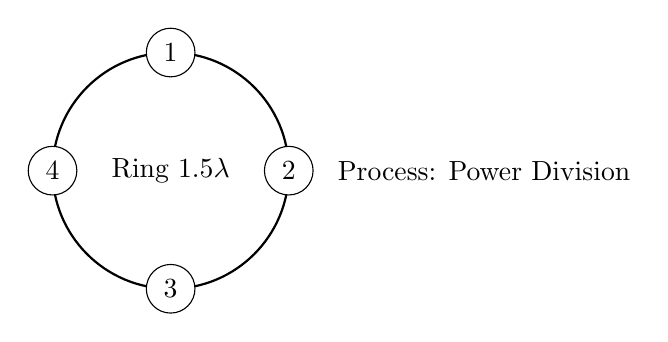
\begin{tikzpicture}
    \draw[thick] (0,0) circle (1.5);
    \node at (0,0) {Ring $1.5\lambda$};
    
    \node[draw, circle, fill=white] (p1) at (90:1.5) {1};
    \node[draw, circle, fill=white] (p2) at (0:1.5) {2};
    \node[draw, circle, fill=white] (p3) at (-90:1.5) {3};
    \node[draw, circle, fill=white] (p4) at (180:1.5) {4};
    
    \node[right] at (2,0) {Process: Power Division};
\end{tikzpicture}
\end{answerdiagram}

\textbf{Working Parameters:}
\begin{itemize}
    \item \keyword{Circumference}: $1.5\lambda$ (Total path length).
    \item \keyword{Spacing}: Ports separated by $\lambda/4$, except one $3\lambda/4$ section.
    \item \keyword{Function}: Input at Port 1 splits equally to 2 and 4. Port 3 is isolated.
\end{itemize}
\end{solutionbox}

\begin{mnemonicbox}
\mnemonic{Ring Runs Round for Power Sharing}
\end{mnemonicbox}

\questionmarks{2(c)}{7}{Explain the construction and working principle of "CIRCULATOR". List its applications.}

\begin{solutionbox}
\textbf{Circulator Construction:}

\begin{answerdiagram}{Three-Port Circulator}
\begin{tikzpicture}[auto, node distance=2cm]
    \node [gtu decision, fill=gray!20] (jun) {Ferrite\\Junction};
    \node [gtu state, above=of jun] (p1) {Port 1};
    \node [gtu state, below right=of jun] (p2) {Port 2};
    \node [gtu state, below left=of jun] (p3) {Port 3};
    
    \draw [gtu arrow] (p1) -- (jun);
    \draw [gtu arrow] (jun) -- (p2);
    \draw [gtu arrow] (p2) |- (jun); % simplified flow representation
    \draw [gtu arrow] (p3) |- (jun);

    % Circular flow arrows
    \draw [->, red, thick] (jun.north) to[bend left] (jun.east);
    \draw [->, red, thick] (jun.east) to[bend left] (jun.south);
    \draw [->, red, thick] (jun.south) to[bend left] (jun.west);
    
    \node at (3,0) {Direction: $1 \rightarrow 2 \rightarrow 3 \rightarrow 1$};
\end{tikzpicture}
\end{answerdiagram}

\textbf{Working Principle:}
\begin{itemize}
    \item Based on \keyword{Faraday Rotation} in ferrite material.
    \item \keyword{Non-reciprocal}: A signal entering Port 1 emerges ONLY at Port 2. Port 2 to Port 3, etc.
    \item Reverse power is blocked (isolated).
\end{itemize}

\textbf{Applications:}
\begin{enumerate}
    \item \keyword{Duplexer in Radar}: Allows single antenna for Tx and Rx.
    \item \keyword{Isolator}: By terminating one port with a matched load.
    \item \keyword{Parametric Amplifiers}: Separation of input and output.
\end{enumerate}
\end{solutionbox}

\begin{mnemonicbox}
\mnemonic{Circulator Circles Clockwise Continuously}
\end{mnemonicbox}

\orquestionmarks{2(a)}{3}{Compare rectangular waveguide and circular waveguide.}

\begin{solutionbox}
\textbf{Comparison:}

\begin{answertable}{Waveguide Comparison}
\begin{tabulary}{\linewidth}{|L|L|L|}
\hline
\textbf{Parameter} & \textbf{Rectangular Waveguide} & \textbf{Circular Waveguide} \\ \hline
\keyword{Cross-section} & Rectangular ($a \times b$) & Circular (radius $a$) \\ \hline
\keyword{Dominant Mode} & $TE_{10}$ & $TE_{11}$ \\ \hline
\keyword{Cutoff Freq} & $f_c = c/2a$ & $f_c = 1.841c/2\pi a$ (Complex) \\ \hline
\keyword{Power Handling} & Lower & Higher \\ \hline
\keyword{Rotation} & Polarization fixed & Supports rotating polarization \\ \hline
\end{tabulary}
\end{answertable}
\end{solutionbox}

\begin{mnemonicbox}
\mnemonic{Rectangles are Regular, Circles are Complex}
\end{mnemonicbox}

\orquestionmarks{2(b)}{4}{Draw and explain the working of a directional coupler.}

\begin{solutionbox}
\textbf{Directional Coupler:}

\begin{answerdiagram}{2-Hole Directional Coupler}
\begin{tikzpicture}[auto, node distance=2cm]
    \node [gtu block, minimum width=4cm] (main) {Main Waveguide};
    \node [gtu block, minimum width=4cm, below=0.5cm of main] (aux) {Auxiliary Waveguide};
    
    \node [left=of main] (p1) {1 (Input)};
    \node [right=of main] (p2) {2 (Through)};
    \node [left=of aux] (p3) {3 (Coupled)};
    \node [right=of aux] (p4) {4 (Isolated)};
    
    \draw [gtu arrow] (p1) -- (main);
    \draw [gtu arrow] (main) -- (p2);
    
    % Coupling holes
    \draw [dashed, ->] (main.south) -- (aux.north);
    \node at (0, -0.25) {Coupling Holes ($\lambda/4$ apart)};
\end{tikzpicture}
\end{answerdiagram}

\textbf{Working:}
\begin{itemize}
    \item Samples a small fraction of forward power into Port 3.
    \item Waves traveling backward towards Port 4 cancel out due to $\lambda/2$ path difference (destructive interference).
\end{itemize}

\textbf{Parameters:}
\begin{itemize}
    \item \keyword{Coupling Factor}: $C = 10 \log(P_1/P_3)$ dB.
    \item \keyword{Directivity}: $D = 10 \log(P_3/P_4)$ dB.
\end{itemize}
\end{solutionbox}

\begin{mnemonicbox}
\mnemonic{Coupler Couples Carefully in Correct Direction}
\end{mnemonicbox}

\orquestionmarks{2(c)}{7}{Explain the construction and working principle of "Travelling Wave Tube". List its applications.}

\begin{solutionbox}
\textbf{Construction:}

\begin{answerdiagram}{Helix TWT}
\begin{tikzpicture}[auto, node distance=1.5cm]
    \node [gtu start] (gun) {Electron\\Gun};
    \node [gtu block, right=of gun, minimum width=4cm] (helix) {Helix Slow-Wave Structure};
    \node [gtu stop, right=of helix] (col) {Collector};
    
    \node [above=of helix] (in) {RF Input};
    \node [above=of col] (out) {RF Output};
    
    \draw [gtu arrow] (gun) -- (helix);
    \draw [gtu arrow] (helix) -- (col);
    
    \draw [->] (in) -- (helix.west);
    \draw [->] (helix.east) -- (out);
    
    \node [below=of helix] {Axial Magnetic Field ($B_0$)};
\end{tikzpicture}
\end{answerdiagram}

\textbf{Working Principle:}
\begin{itemize}
    \item \keyword{Slow Wave Structure}: Helix reduces RF phase velocity to match electron beam velocity ($v_{ph} \approx v_e$).
    \item \keyword{Interaction}: Continuous interaction bunches electrons. Kinetic energy is transferred from electrons to the RF field.
    \item \keyword{Amplification}: Signal grows exponentially along the tube.
\end{itemize}

\textbf{Applications:}
\begin{itemize}
    \item Satellite Transponders (High Reliability).
    \item Radar Systems (Wide Bandwidth).
    \item Electronic Warfare (Jamming).
\end{itemize}
\end{solutionbox}

\begin{mnemonicbox}
\mnemonic{TWT Transfers Tremendous power Through Travel}
\end{mnemonicbox}

\questionmarks{3(a)}{3}{Explain the Indirect method for higher VSWR measurement.}

\begin{solutionbox}
\textbf{Double Minimum Method (Indirect):}
Used when VSWR > 10. Direct reading is inaccurate.

\textbf{Procedure:}
\begin{enumerate}
    \item Find position of voltage minimum ($V_{min}$).
    \item Move probe left and right to points where power is double ($2 \times V_{min}^2$).
    \item Measure distance $d$ between these "double power" points.
\end{enumerate}

\textbf{Formula:}
\[ VSWR = \frac{\lambda_g}{\pi d} \]
Where $\lambda_g$ is guide wavelength and $d$ is width of minimum at 3dB points.
\end{solutionbox}

\begin{mnemonicbox}
\mnemonic{Indirect method uses Intermediate Attenuation}
\end{mnemonicbox}

\questionmarks{3(b)}{4}{Write and explain the frequency limitations of conventional tubes.}

\begin{solutionbox}
\textbf{Conventional Tube Limitations at Microwave Frequencies:}

\begin{answertable}{Limitations and Effects}
\begin{tabulary}{\linewidth}{|L|L|}
\hline
\textbf{Limitation} & \textbf{Effect} \\ \hline
\keyword{Transit Time} & Time for electron to cross gap becomes comparable to RF period. Causes Conductance ($G$) loading and grid heating. \\ \hline
\keyword{Lead Inductance} & $X_L = 2\pi f L$. High impedance in cathode lead reduces effective gain. \\ \hline
\keyword{Interelectrode Capacitance} & $X_C = 1/2\pi f C$. Shunts RF signal, reducing output impedance and gain. \\ \hline
\keyword{Skin Effect} & Current restricted to surface, increasing resistance and losses. \\ \hline
\end{tabulary}
\end{answertable}

\textbf{Result:} Gain drops to zero, and noise increases.
\end{solutionbox}

\begin{mnemonicbox}
\mnemonic{Transit Time Troubles Traditional Tubes}
\end{mnemonicbox}

\questionmarks{3(c)}{7}{Explain construction and working of Two cavity klystron with applegate diagram. List its advantages.}

\begin{solutionbox}
\textbf{Two Cavity Klystron:}

\begin{answerdiagram}{Klystron Amplifier}
\begin{tikzpicture}[auto, node distance=1.5cm]
    \node [gtu start] (k) {K};
    \node [gtu block, right=of k] (buncher) {Buncher\\Grid};
    \node [gtu block, right=of buncher, minimum width=2.5cm] (drift) {Drift Space};
    \node [gtu block, right=of drift] (catcher) {Catcher\\Grid};
    \node [gtu stop, right=of catcher] (col) {Collector};
    
    \draw [gtu arrow] (k) -- (buncher);
    \draw [gtu arrow] (buncher) -- (drift);
    \draw [gtu arrow] (drift) -- (catcher);
    \draw [gtu arrow] (catcher) -- (col);
    
    \node [above=of buncher] {RF In};
    \node [above=of catcher] {RF Out};
\end{tikzpicture}
\end{answerdiagram}

\textbf{Applegate Diagram (Bunching):}

\begin{answerdiagram}{Applegate Diagram}
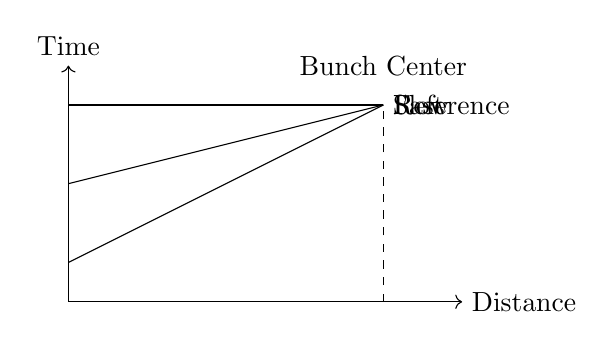
\begin{tikzpicture}
    \draw[->] (0,0) -- (5,0) node[right] {Distance};
    \draw[->] (0,0) -- (0,3) node[above] {Time};
    
    % Electron trajectories meeting at a point
    \draw (0,0.5) -- (4,2.5) node[right] {Slow};
    \draw (0,1.5) -- (4,2.5) node[right] {Reference};
    \draw (0,2.5) -- (4,2.5) node[right] {Fast};
    
    \node at (4,3) {Bunch Center};
    \draw[dashed] (4,0) -- (4,2.5);
\end{tikzpicture}
\end{answerdiagram}

\textbf{Working:}
\begin{enumerate}
    \item \keyword{Velocity Modulation}: RF input in Buncher cavity accelerates/decelerates electrons.
    \item \keyword{Bunching}: In drift space, fast electrons catch up to slow ones.
    \item \keyword{Current Modulation}: Electron bunches induce strong RF current in Catcher cavity.
\end{enumerate}

\textbf{Advantages:} High Gain (>30dB), High Power, Stable.
\end{solutionbox}

\begin{mnemonicbox}
\mnemonic{Klystron Kicks with Kinetic Bunching}
\end{mnemonicbox}

\orquestionmarks{3(a)}{3}{Explain construction and working of BWO.}

\begin{solutionbox}
\textbf{Backward Wave Oscillator (BWO):}
A TWT-like device where wave travels opposite to electron beam.

\textbf{Construction:}
Similar to TWT (Electron gun, Helix), but RF output is taken near the gun end.

\textbf{Working:}
\begin{itemize}
    \item Beam interacts with \keyword{backward space harmonic} of the wave.
    \item Feedback is internal (wave flows back to input).
    \item \keyword{Voltage Tuning}: Oscillation frequency controlled by beam voltage.
\end{itemize}
\end{solutionbox}

\begin{mnemonicbox}
\mnemonic{BWO goes Backward While Oscillating}
\end{mnemonicbox}

\orquestionmarks{3(b)}{4}{Explain hazards due to microwave radiation.}

\begin{solutionbox}
\textbf{Microwave Hazards:}

\begin{itemize}
    \item \keyword{HERP}: Hazards of EM Radiation to Personnel (Biological damage).
    \item \keyword{HERO}: Hazards to Ordnance (Explosives detonation).
    \item \keyword{HERF}: Hazards to Fuel (Ignition of vapors).
\end{itemize}

\textbf{Biological Effects:}
\begin{itemize}
    \item \keyword{Thermal}: Heating of water-rich tissues (eyes, brain, stomach). Can cause cataracts.
    \item \keyword{Non-thermal}: Nervous system effects (debated).
\end{itemize}

\textbf{Safety Limit}: Generally $< 10 mW/cm^2$.
\end{solutionbox}

\begin{mnemonicbox}
\mnemonic{Microwaves Make Multiple Medical Maladies}
\end{mnemonicbox}

\orquestionmarks{3(c)}{7}{Explain construction and working of magnetron with neat sketch. List its applications.}

\begin{solutionbox}
\textbf{Magnetron Construction:}

\begin{answerdiagram}{Magnetron Cross-Section}
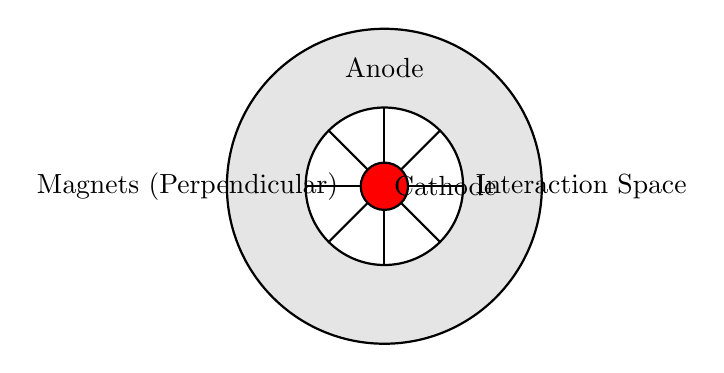
\begin{tikzpicture}
    % Anode Block
    \draw[thick, fill=gray!20] (0,0) circle (2);
    \draw[thick, fill=white] (0,0) circle (1);
    
    % Cavities (Simplified Vanes)
    \foreach \angle in {0,45,...,315}
    {
        \draw[thick] (0,0) -- (\angle:1);
    }
    
    % Cathode
    \draw[thick, fill=red] (0,0) circle (0.3);
    \node at (0,0) [right] {Cathode};
    
    \node at (0,1.5) {Anode};
    \node at (2.5,0) {Interaction Space};
    \node at (-2.5,0) {Magnets (Perpendicular)};
\end{tikzpicture}
\end{answerdiagram}

\textbf{Working Principle:}
\begin{itemize}
    \item \keyword{Crossed Fields}: Radial Electric field ($E$) and Axial Magnetic field ($B$).
    \item \keyword{Electron Motion}: Electrons spiral outwards in cycloid paths.
    \item \keyword{Phase Focusing}: Electrons transfer energy to RF fields in the cavities ("spokes" of charge).
    \item \keyword{$\pi$-mode}: Adjacent cavities are $180^\circ$ out of phase.
\end{itemize}

\textbf{Applications:} Microwave Ovens, Radar Transmitters.
\end{solutionbox}

\begin{mnemonicbox}
\mnemonic{Magnetron Makes Microwaves Magnificently}
\end{mnemonicbox}

\questionmarks{4(a)}{3}{Explain working of P-i-N diode.}

\begin{solutionbox}
\textbf{P-i-N Diode Working:}
Has an \keyword{Intrinsic (I)} layer between P and N regions.

\begin{answerdiagram}{PIN Diode Structure}
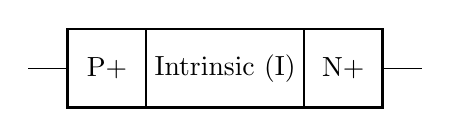
\begin{tikzpicture}
    \draw[thick] (0,0) rectangle (4,1);
    \draw[thick] (1,0) -- (1,1);
    \draw[thick] (3,0) -- (3,1);
    \node at (0.5,0.5) {P+};
    \node at (2,0.5) {Intrinsic (I)};
    \node at (3.5,0.5) {N+};
    \draw (0,0.5) -- (-0.5,0.5);
    \draw (4,0.5) -- (4.5,0.5);
\end{tikzpicture}
\end{answerdiagram}

\textbf{States:}
\begin{enumerate}
    \item \keyword{Forward Bias}: Injection of carriers lowers resistance ($R \approx 1\Omega$). Acts as \keyword{Short}.
    \item \keyword{Reverse Bias}: Carriers swept out, high resistance ($R > 10k\Omega$). Acts as \keyword{Open}.
\end{enumerate}

\textbf{Applications}: RF Switch, Variable Attenuator.
\end{solutionbox}

\begin{mnemonicbox}
\mnemonic{PIN controls Power IN Networks}
\end{mnemonicbox}

\questionmarks{4(b)}{4}{Explain the working of Varactor diode with sketch.}

\begin{solutionbox}
\textbf{Varactor Diode:}
Operates as a \keyword{voltage-controlled capacitor}.

\begin{answerdiagram}{Varactor C-V Curve}
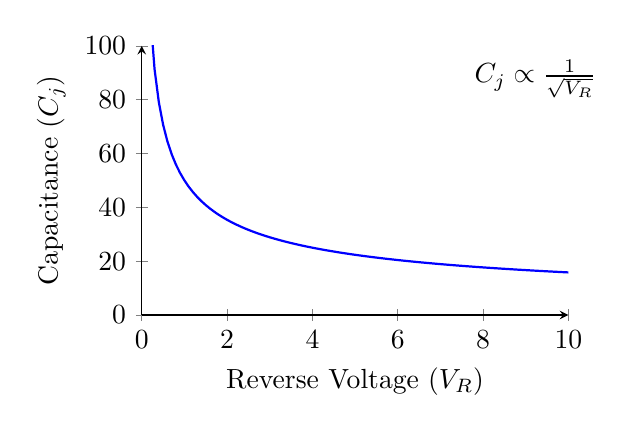
\begin{tikzpicture}
    \begin{axis}[
        axis lines = left,
        xlabel = {Reverse Voltage ($V_R$)},
        ylabel = {Capacitance ($C_j$)},
        ymin=0, ymax=100,
        xmin=0, xmax=10,
        height=5cm, width=7cm
    ]
    \addplot [domain=0.1:10, samples=100, blue, thick] {50/sqrt(x)};
    \end{axis}
    \node at (5,3) {$C_j \propto \frac{1}{\sqrt{V_R}}$};
\end{tikzpicture}
\end{answerdiagram}

\textbf{Working:}
\begin{itemize}
    \item \keyword{Reverse Bias}: Widens depletion region $\rightarrow$ Decreases Capacitance.
    \item \keyword{Tuning}: Changing voltage changes $C$, which changes resonant frequency $f = 1/2\pi\sqrt{LC}$.
\end{itemize}
\end{solutionbox}

\begin{mnemonicbox}
\mnemonic{Varactor Varies Capacitance with Voltage}
\end{mnemonicbox}

\questionmarks{4(c)}{7}{Explain construction and working of Tunnel Diode and explain tunneling phenomenon in detail. List its applications.}

\begin{solutionbox}
\textbf{Tunnel Diode Construction:}
\begin{itemize}
    \item \keyword{Heavily Doped}: ($10^{19}$ atoms/cm$^3$). Degenerate P and N regions.
    \item \keyword{Thin Junction}: Narrow depletion width (~100 \AA).
\end{itemize}

\textbf{Tunneling Phenomenon:}
Quantum mechanical effect where electrons punch through the potential barrier instead of climbing over it, due to wave-like nature and narrow barrier.

\begin{answerdiagram}{Tunnel Diode I-V}
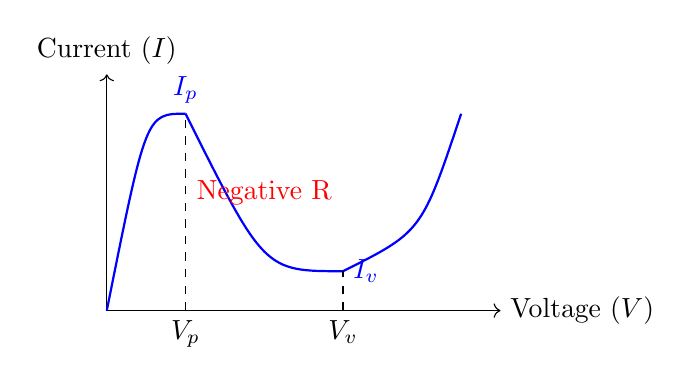
\begin{tikzpicture}
    \draw[->] (0,0) -- (5,0) node[right] {Voltage ($V$)};
    \draw[->] (0,0) -- (0,3) node[above] {Current ($I$)};
    
    \draw[blue, thick] (0,0) .. controls (0.5,2.5) .. (1,2.5); % Peak
    \draw[blue, thick] (1,2.5) node[above] {$I_p$} -- (1,2.5) .. controls (2,0.5) .. (3,0.5); % Negative R
    \draw[blue, thick] (3,0.5) node[right] {$I_v$} .. controls (4,1) .. (4.5,2.5); % Exponential
    
    \draw[dashed] (1,0) node[below] {$V_p$} -- (1,2.5);
    \draw[dashed] (3,0) node[below] {$V_v$} -- (3,0.5);
    
    \node[red] at (2,1.5) {Negative R};
\end{tikzpicture}
\end{answerdiagram}

\textbf{Working Regions:}
\begin{enumerate}
    \item \keyword{Peak Point ($V_p$)}: Max tunneling current.
    \item \keyword{Negative Resistance ($V_p$ to $V_v$)}: Current decreases as voltage increases. Used for oscillators.
    \item \keyword{Valley Point ($V_v$)}: Tunneling ceases.
\end{enumerate}

\textbf{Applications}: Oscillators, High speed switching.
\end{solutionbox}

\begin{mnemonicbox}
\mnemonic{Tunnel Diode Tunnels Through barriers Terrifically}
\end{mnemonicbox}

\orquestionmarks{4(a)}{3}{Describe the operation of IMPATT diode.}

\begin{solutionbox}
\textbf{IMPATT Diode (Impact Avalanche Transit Time):}
Generates microwave power using:
\begin{enumerate}
    \item \keyword{Impact Ionization}: Avalanche multiplication creates carriers (90$^\circ$ phase shift).
    \item \keyword{Transit Time}: Drift of carriers through region adds remaining 90$^\circ$ shift.
\end{enumerate}
Total 180$^\circ$ phase delay results in \keyword{Negative Resistance}.

\textbf{Key Stats}: High Power, High Noise, Breakdown voltage ~100V.
\end{solutionbox}

\begin{mnemonicbox}
\mnemonic{IMPATT Impacts with Avalanche Transit Time}
\end{mnemonicbox}

\orquestionmarks{4(b)}{4}{Explain the frequency up and down conversion concepts for parametric amplifier.}

\begin{solutionbox}
\textbf{Parametric Amplifier Conversion:}
Uses a nonlinear reactance (Varactor) pumped at frequency $f_p$.

\textbf{Up-Conversion:}
\begin{itemize}
    \item Input: $f_s$ (Signal).
    \item Output: $f_o = f_p + f_s$ (Sum frequency) or $f_p - f_s$.
    \item \keyword{Gain}: Power gain proportional to frequency ratio ($f_o/f_s$). Stable with low noise.
\end{itemize}

\textbf{Down-Conversion:}
\begin{itemize}
    \item Output: $f_o = f_p - f_s$.
    \item \keyword{Negative Resistance}: Can lead to instability/oscillation.
\end{itemize}
\end{solutionbox}

\begin{mnemonicbox}
\mnemonic{Parametric Pump Provides frequency conversion Plus gain}
\end{mnemonicbox}

\orquestionmarks{4(c)}{7}{Describe the construction and working principle of RUBY MASER. List its applications.}

\begin{solutionbox}
\textbf{Ruby Maser:}

\begin{answerdiagram}{Maser Block Diagram}
\begin{tikzpicture}[auto, node distance=1.5cm]
    \node [gtu block, fill=red!10] (ruby) {Ruby Crystal};
    \node [gtu start, above=of ruby] (pump) {Pump Source};
    \node [gtu input, left=of ruby] (sig) {Signal In};
    \node [gtu output, right=of ruby] (out) {Amplified Out};
    \node [below=0.5cm of ruby] (cool) {Liquid Helium (4.2K)};
    \node [right=0.5cm of cool] (mag) {Magnet ($B$)};
    
    \draw [gtu arrow] (pump) -- (ruby);
    \draw [gtu arrow] (sig) -- (ruby);
    \draw [gtu arrow] (ruby) -- (out);
\end{tikzpicture}
\end{answerdiagram}

\textbf{Working Principle (Stimulated Emission):}
\begin{enumerate}
    \item \keyword{Population Inversion}: Pump energy raises electrons to unstable higher energy level ($E_3$).
    \item \keyword{Stimulated Emission}: Incoming signal photons ($E_2$) trigger electrons to drop level, releasing coherent photons.
    \item \keyword{Cooling}: Liquid Helium reduces thermal noise.
\end{enumerate}

\textbf{Applications:} Deep space communication (NASA), Radio Astronomy.
\end{solutionbox}

\begin{mnemonicbox}
\mnemonic{RUBY MASER Makes Amazingly Sensitive Electromagnetic Receivers}
\end{mnemonicbox}

\questionmarks{5(a)}{3}{Draw and explain the functional block diagram of MTI RADAR.}

\begin{solutionbox}
\textbf{MTI (Moving Target Indication) Radar:}

\begin{answerdiagram}{MTI Radar}
\begin{tikzpicture}[auto, node distance=1.5cm]
    \node [gtu block] (tx) {Tx};
    \node [gtu block, right=of tx] (dup) {Duplexer};
    \node [gtu input, right=of dup] (ant) {Ant};
    \node [gtu block, below=of tx] (mix) {Mixer};
    \node [gtu block, below=of mix] (pd) {Phase Det};
    \node [gtu block, right=of pd] (dl) {Delay Line};
    \node [gtu block, right=of dl] (sub) {Subtractor};
    
    \node [gtu block, left=of mix] (stalo) {STALO};
    \node [gtu block, left=of pd] (coho) {COHO};
    
    \draw [gtu arrow] (tx) -- (dup);
    \draw [gtu arrow] (dup) -- (ant);
    \draw [gtu arrow] (dup) -- (mix);
    \draw [gtu arrow] (stalo) -- (mix);
    \draw [gtu arrow] (mix) -- (pd);
    \draw [gtu arrow] (coho) -- (pd);
    
    \draw [gtu arrow] (pd) -- (dl);
    \draw [gtu arrow] (pd) -- node[above] {} (sub);
    \draw [gtu arrow] (dl) -- (sub);
    
    \node [right=0.5cm of sub] {To Scope};
    \draw [->] (sub) -- +(1,0);
\end{tikzpicture}
\end{answerdiagram}

\textbf{Function:} Separates moving targets from clutter (fixed targets) using Doppler phase shift comparison between pulses.
\end{solutionbox}

\begin{mnemonicbox}
\mnemonic{MTI Makes Targets Intelligible by Motion}
\end{mnemonicbox}

\questionmarks{5(b)}{4}{Compare RADAR with SONAR.}

\begin{solutionbox}
\textbf{Comparison:}

\begin{answertable}{Radar vs Sonar}
\begin{tabulary}{\linewidth}{|L|L|L|}
\hline
\textbf{Parameter} & \textbf{RADAR} & \textbf{SONAR} \\ \hline
\keyword{Wave} & EM Waves (Microwaves) & Acoustic (Sound) Waves \\ \hline
\keyword{Speed} & $3 \times 10^8$ m/s & ~1500 m/s \\ \hline
\keyword{Medium} & Air, Vacuum & Water \\ \hline
\keyword{Range} & Long (Space/Air) & Short (Underwater) \\ \hline
\keyword{Use} & Tracking Aircrafts & Submarines, Fish finding \\ \hline
\end{tabulary}
\end{answertable}
\end{solutionbox}

\begin{mnemonicbox}
\mnemonic{RADAR Radiates, SONAR Sounds}
\end{mnemonicbox}

\questionmarks{5(c)}{7}{Obtain the equation of maximum RADAR range. Explain the factors affecting the maximum radar range.}

\begin{solutionbox}
\textbf{Radar Range Equation:}

\[ R_{max} = \left[ \frac{P_t G^2 \lambda^2 \sigma}{(4\pi)^3 P_{min}} \right]^{1/4} \]

\textbf{Derivation:}
\begin{enumerate}
    \item Power density at target R: $\frac{P_t G}{4\pi R^2}$.
    \item Power reflected by target ($\sigma$): $\frac{P_t G \sigma}{4\pi R^2}$.
    \item Power density at receiver (return path): $\frac{P_t G \sigma}{(4\pi R^2)^2}$.
    \item Effective Area of Antenna $A_e = \frac{G \lambda^2}{4\pi}$.
    \item Received Power $P_r = \text{Density} \times A_e = \frac{P_t G^2 \lambda^2 \sigma}{(4\pi)^3 R^4}$.
    \item Set $P_r = P_{min}$ and solve for $R$.
\end{enumerate}

\textbf{Factors Affecting Range:}
\begin{itemize}
    \item \keyword{Transmitter Power ($P_t$)}: $R \propto P_t^{1/4}$. Need huge power increase for small range gain.
    \item \keyword{Antenna Gain ($G$) / Area}: Larger antenna improves range.
    \item \keyword{Target RCS ($\sigma$)}: Bigger/metallic targets are easier to see.
    \item \keyword{Min Detectable Signal ($P_{min}$)}: Better receiver sensitivity increases range.
\end{itemize}
\end{solutionbox}


\orquestionmarks{5(a)}{3}{Describe the Doppler effect in CW Doppler RADAR.}

\begin{solutionbox}
\textbf{Doppler Effect:}
The \keyword{frequency shift} observed when a target moves relative to the RADAR.

\textbf{Formula:}
\[ f_d = \frac{2 V_r f_0}{c} = \frac{2 V_r}{\lambda} \]
Where:
\begin{itemize}
    \item $V_r$: Radial velocity (m/s).
    \item $f_0$: Transmitted frequency.
    \item $c$: Speed of light.
\end{itemize}

\textbf{Shift Direction:}
\begin{itemize}
    \item \keyword{Approaching}: $f_r > f_0$ (Positive shift).
    \item \keyword{Receding}: $f_r < f_0$ (Negative shift).
\end{itemize}
\end{solutionbox}

\begin{mnemonicbox}
\mnemonic{Doppler Detects Direction with Doubled frequency shift}
\end{mnemonicbox}

\orquestionmarks{5(b)}{4}{Explain PPI Display method for RADAR}

\begin{solutionbox}
\textbf{PPI (Plan Position Indicator):}
Displays a \keyword{top-down map view} of the radar coverage.

\begin{answerdiagram}{PPI Display}
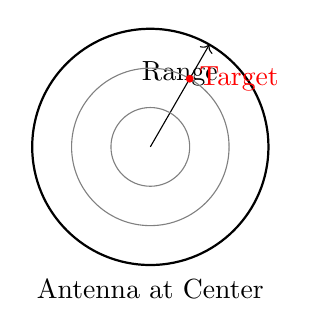
\begin{tikzpicture}
    \draw[thick] (0,0) circle (1.5);
    \draw[->] (0,0) -- (60:1.5) node[midway, above] {Range};
    \foreach \r in {0.5, 1.0} \draw[gray] (0,0) circle (\r);
    \fill[red] (60:1.0) circle (0.05) node[right] {Target};
    \node at (0,-1.8) {Antenna at Center};
\end{tikzpicture}
\end{answerdiagram}

\textbf{Features:}
\begin{enumerate}
    \item \keyword{Center}: Radar location.
    \item \keyword{Angle}: Target Azimuth (Bearing).
    \item \keyword{Radius}: Target Range (Distance).
    \item \keyword{Sweep}: Rotating trace synchronized with antenna.
\end{enumerate}
\end{solutionbox}

\begin{mnemonicbox}
\mnemonic{PPI Provides Position Information Perfectly}
\end{mnemonicbox}

\orquestionmarks{5(c)}{7}{Draw the block diagram of Pulse radar and explain the working principle.}

\begin{solutionbox}
\textbf{Pulse Radar Block Diagram:}

\begin{answerdiagram}{Pulse Radar}
\begin{tikzpicture}[auto, node distance=1.5cm]
    \node [gtu start] (timer) {Timer};
    \node [gtu block, right=of timer] (mod) {Modulator};
    \node [gtu block, right=of mod] (tx) {Transmitter};
    \node [gtu block, right=of tx] (dup) {Duplexer};
    \node [gtu input, right=of dup] (ant) {Antenna};
    
    \node [gtu block, below=of dup] (rx) {Receiver};
    \node [gtu stop, left=of rx] (disp) {Display};
    
    \draw [gtu arrow] (timer) -- (mod);
    \draw [gtu arrow] (mod) -- (tx);
    \draw [gtu arrow] (tx) -- (dup);
    \draw [gtu arrow] (dup) -- (ant);
    \draw [gtu arrow] (dup) -- (rx);
    \draw [gtu arrow] (rx) -- (disp);
    \draw [gtu arrow] (timer) -| (disp); % Sync
\end{tikzpicture}
\end{answerdiagram}

\textbf{Working Principle:}
\begin{itemize}
    \item \keyword{Transmission}: High power pulses emitted at regular intervals (PRF).
    \item \keyword{Reception}: Echoes received during "listening" time.
    \item \keyword{Duplexer}: Protects receiver during transmission; routes echo to receiver.
    \item \keyword{Timing}: Distance calculated from time delay $T$: $R = cT/2$.
\end{itemize}
\end{solutionbox}

\begin{mnemonicbox}
\mnemonic{Pulse RADAR Pulses Powerfully for Precise Position}
\end{mnemonicbox}

\end{document}
